% ============================================================================
% Regression lecture 2 of 3: residual analysis and diagnostics; regression
% performance measures
% Needs: booktabs
% R code of every figure: in the comments above its \includegraphics
% R packages for the figures: tidyverse, patchwork, ISLR2 (R >= 4.1, ggplot2 >= 3.5)
% Figures (figures/): reg_diag_four, reg_diag_nonlinear, reg_diag_autocorr,
%   reg_diag_variance, reg_diag_outlier, reg_diag_leverage, reg_credit_collinearity,
%   reg_junk_r2 (new), reg_train_test
% Running examples: Advertising (additive vs interaction model), Auto (mpg on
%   horsepower, weight, year), Credit (collinearity)
% ============================================================================

\section{Residual Analysis and Diagnostics}

\begin{frame}{Learning outcomes}
    \begin{itemize}
        \item State the assumptions behind least squares inference and explain how residuals reveal violations
        \item Compute and interpret standardized residuals and leverage from the hat matrix
        \item Diagnose and remedy non-linearity, correlated errors, non-constant variance, outliers, high-leverage observations and collinearity
        \item Compute and interpret MSE, RMSE, MAE, RSE, $R^2$ and adjusted $R^2$
        \item Distinguish training error from test error
    \end{itemize}
\end{frame}

\begin{frame}{Residuals and model assumptions}
    \begin{itemize}
        \item Residual vector $\mathbf{e} = \mathbf{y} - \hat{\mathbf{y}}$ with entries $e^{(i)} = y^{(i)} - \hat{y}^{(i)}$; least squares gives $\tilde{\mathbf{X}}^\top \mathbf{e} = \mathbf{0}$, so the residuals sum to zero and are uncorrelated with every feature
        \item Standard errors, confidence and prediction intervals, and tests rely on assumptions about the errors: the relationship is linear in the coefficients, the errors $\varepsilon^{(i)}$ are uncorrelated, they have constant variance $\sigma^2$, and (for exact small-sample inference) they are normal
        \item \textbf{Residual analysis} checks these assumptions with plots; the main tool is the plot of residuals against fitted values: random scatter around zero is good, a curve signals non-linearity, a funnel signals non-constant variance
        \item Three further problems: outliers, high-leverage observations, and collinearity
    \end{itemize}
\end{frame}

\begin{frame}{Residuals and the hat matrix}
    \begin{itemize}
        \item Fitted values and residuals are linear functions of the labels: $\hat{\mathbf{y}} = \mathbf{H}\mathbf{y}$ and $\mathbf{e} = (\mathbf{I} - \mathbf{H})\mathbf{y}$, with the \textbf{hat matrix} $\mathbf{H} = \tilde{\mathbf{X}} (\tilde{\mathbf{X}}^\top \tilde{\mathbf{X}})^{-1} \tilde{\mathbf{X}}^\top$ (symmetric, idempotent, $\mathrm{tr}(\mathbf{H}) = p+1$)
        \item Since $(\mathbf{I} - \mathbf{H})\tilde{\mathbf{X}} = \mathbf{0}$, the residuals depend on the errors only: $\mathbf{e} = (\mathbf{I} - \mathbf{H})\symbf{\varepsilon}$
        \item Hence $\mathbb{E}[\mathbf{e}] = \mathbf{0}$ and $\mathrm{Cov}(\mathbf{e}) = \sigma^2 (\mathbf{I} - \mathbf{H})$; reading off the diagonal,
    \end{itemize}
    \[
        \mathrm{Var}\big(e^{(i)}\big) = \sigma^2 \big(1 - h^{(i)}\big), \qquad h^{(i)} = H_{ii}
    \]
    \begin{itemize}
        \item Even when all errors have the same variance, the residuals do not: observations with large \textbf{leverage} $h^{(i)}$ have residuals with smaller variance, because the fit is pulled towards them; the leverages add up to $\sum_i h^{(i)} = p+1$
    \end{itemize}
\end{frame}

\begin{frame}{Standardized (studentized) residuals}
    \begin{itemize}
        \item Raw residuals have unequal variances and carry the units of $y$; dividing by the estimated standard deviation fixes both:
    \end{itemize}
    \[
        r^{(i)} = \frac{e^{(i)}}{\hat\sigma \sqrt{1 - h^{(i)}}}, \qquad \hat\sigma = \mathrm{RSE}
    \]
    \begin{itemize}
        \item Each $r^{(i)}$ has variance close to 1 and no units, so residuals can be compared across observations and across models
        \item With normal errors about 99.7\% of the $r^{(i)}$ fall within $\pm 3$: an observation with $|r^{(i)}| > 3$ is unusual, but among 400 observations one such value is expected by chance
        \item ISLP calls $r^{(i)}$ the studentized residual; in R it is computed by \texttt{rstandard()}
    \end{itemize}
\end{frame}

\mode<article>{
    \paragraph{Externally studentized residuals.}
    A variant replaces $\hat\sigma$ by $\hat\sigma_{(i)}$, the estimate computed with observation $i$ left out. It removes the influence of a suspicious point on its own residual and follows a $t_{n-p-2}$ distribution exactly under normal errors. In R this is \texttt{rstudent()}; for moderate $n$ the two versions rarely lead to different conclusions.
}

\begin{frame}[allowframebreaks]{Four standard diagnostic plots}
    \begin{columns}[T]
        \begin{column}{0.40\textwidth}
            \begin{itemize}
                \item \textbf{Residuals vs fitted}: curve = non-linearity, funnel = non-constant variance
                \item \textbf{Normal QQ plot}: points near the line = roughly normal errors
                \item \textbf{Scale-location}: upward trend = non-constant variance
                \item \textbf{Residuals vs leverage}: flags unusual observations
                \item Shown: Auto, mpg on horsepower, weight and year
            \end{itemize}
        \end{column}
        \begin{column}{0.58\textwidth}
            % ---- R code: figures/reg_diag_four.pdf ----
            % library(tidyverse)
            % library(patchwork)
            % library(ISLR2)                      # Auto data
            % theme_set(theme_minimal(base_size = 8) +
            %             theme(plot.title = element_text(size = 8, face = "bold"),
            %                   plot.background = element_rect(fill = "transparent", colour = NA),
            %                   panel.background = element_rect(fill = "transparent", colour = NA),
            %                   legend.background = element_rect(fill = "transparent", colour = NA)))
            % dir.create("figures", showWarnings = FALSE)
            %
            % fit <- lm(mpg ~ horsepower + weight + year, data = Auto)
            % dg <- tibble(fitted = fitted(fit), resid = resid(fit),
            %              std = rstandard(fit), lev = hatvalues(fit))
            % pts <- geom_point(size = 0.4, alpha = 0.6, colour = "grey30")
            %
            % p1 <- ggplot(dg, aes(fitted, resid)) + pts +
            %   geom_hline(yintercept = 0, linetype = "dashed") +
            %   labs(title = "residuals vs fitted", x = "fitted values", y = "residuals")
            % p2 <- ggplot(dg, aes(sample = std)) +
            %   stat_qq(size = 0.4, alpha = 0.6) + stat_qq_line(colour = "red", linewidth = 0.4) +
            %   labs(title = "normal QQ plot", x = "theoretical quantiles", y = "standardized residuals")
            % p3 <- ggplot(dg, aes(fitted, sqrt(abs(std)))) + pts +
            %   labs(title = "scale-location", x = "fitted values", y = "sqrt |standardized residual|")
            % p4 <- ggplot(dg, aes(lev, std)) + pts +
            %   geom_hline(yintercept = c(-3, 0, 3), linetype = "dashed") +
            %   labs(title = "residuals vs leverage", x = "leverage", y = "standardized residuals")
            %
            % p <- (p1 | p2) / (p3 | p4)
            % ggsave("figures/reg_diag_four.pdf", p, width = 4.4, height = 2.75, bg = "transparent")
            \begin{center}
                
\includegraphics[width=\linewidth]{figures/reg_diag_four.pdf}
            \end{center}
        \end{column}
    \end{columns}
\end{frame}

\begin{frame}[allowframebreaks]{Problem 1: non-linearity}
    \begin{itemize}
        \item If the true relationship is non-linear, predictions and inference are unreliable; the residual plot shows a pattern, often a U-shape
        \item Advertising, additive TV + radio model: positive residuals at the smallest and largest fitted values, negative in between, a sign of missing synergy
        \item With the TV $\times$ radio interaction the curvature weakens and RSE falls from 1.68 to 0.94; a few large negative residuals remain
        \item Remedies: transform features ($\log x$, $\sqrt{x}$), add interaction terms, or fit a more flexible model
    \end{itemize}
    % ---- R code: figures/reg_diag_nonlinear.pdf ----
    % library(tidyverse)
    % theme_set(theme_minimal(base_size = 9) +
    %             theme(plot.title = element_text(size = 9, face = "bold"),
    %                   plot.background = element_rect(fill = "transparent", colour = NA),
    %                   panel.background = element_rect(fill = "transparent", colour = NA),
    %                   legend.background = element_rect(fill = "transparent", colour = NA)))
    % dir.create("figures", showWarnings = FALSE)
    %
    % adv_url <- "https://raw.githubusercontent.com/JWarmenhoven/ISLR-python/master/Notebooks/Data/Advertising.csv"
    % ad <- read_csv(adv_url, show_col_types = FALSE) |> select(-1)
    %
    % fit_add <- lm(Sales ~ TV + Radio, data = ad)
    % fit_int <- lm(Sales ~ TV * Radio, data = ad)
    % res <- bind_rows(tibble(fitted = fitted(fit_add), resid = resid(fit_add), model = "additive: TV + radio"),
    %                  tibble(fitted = fitted(fit_int), resid = resid(fit_int), model = "with TV x radio interaction"))
    %
    % p <- ggplot(res, aes(fitted, resid)) +
    %   geom_point(size = 0.5, alpha = 0.6, colour = "grey30") +
    %   geom_hline(yintercept = 0, linetype = "dashed") +
    %   facet_wrap(~ model) +
    %   labs(x = "fitted values", y = "residuals")
    % ggsave("figures/reg_diag_nonlinear.pdf", p, width = 6.0, height = 2.75, bg = "transparent")
    \begin{center}
        
\includegraphics[width=0.95\linewidth]{figures/reg_diag_nonlinear.pdf}
    \end{center}
\end{frame}

\begin{frame}[allowframebreaks]{Problem 2: correlated errors}
    \begin{itemize}
        \item The errors are assumed uncorrelated; this fails for time series (neighbouring errors alike) and for repeated measurements on the same unit
        \item Consequence: standard errors are too small, so intervals are too narrow and $p$-values too small
        \item Detection: plot residuals in observation order; tracking (neighbouring residuals alike) signals positive correlation ($\rho$ = correlation of successive errors)
        \item Remedy: time-series or mixed models (out of the scope this lecture)
    \end{itemize}
    % ---- R code: figures/reg_diag_autocorr.pdf ----
    % library(tidyverse)
    % theme_set(theme_minimal(base_size = 9) +
    %             theme(plot.title = element_text(size = 9, face = "bold"),
    %                   plot.background = element_rect(fill = "transparent", colour = NA),
    %                   panel.background = element_rect(fill = "transparent", colour = NA),
    %                   legend.background = element_rect(fill = "transparent", colour = NA)))
    % dir.create("figures", showWarnings = FALSE)
    %
    % set.seed(3)
    % n <- 100
    % ar1 <- function(rho) {                      # autocorrelated errors: e_t = rho * e_(t-1) + u_t
    %   e <- numeric(n); u <- rnorm(n); e[1] <- u[1]
    %   for (k in 2:n) e[k] <- rho * e[k - 1] + u[k]
    %   e
    % }
    % res <- map_dfr(c(0, 0.5, 0.9), function(rho) {
    %   d <- tibble(t = 1:n, y = 1 + 0.05 * (1:n) + ar1(rho))
    %   tibble(t = d$t, resid = resid(lm(y ~ t, data = d)), panel = paste("rho =", rho))
    % })
    %
    % p <- ggplot(res, aes(t, resid)) +
    %   geom_hline(yintercept = 0, linetype = "dashed") +
    %   geom_line(linewidth = 0.3) +
    %   geom_point(size = 0.4) +
    %   facet_wrap(~ panel) +
    %   labs(x = "observation order", y = "residual")
    % ggsave("figures/reg_diag_autocorr.pdf", p, width = 6.0, height = 2.75, bg = "transparent")
    \begin{center}
        
\includegraphics[width=0.95\linewidth]{figures/reg_diag_autocorr.pdf}
    \end{center}
\end{frame}

\begin{frame}[allowframebreaks]{Problem 3: non-constant variance}
    \begin{itemize}
        \item \textbf{Heteroscedasticity}: $\mathrm{Var}(\varepsilon^{(i)})$ changes with the level of the response (a funnel in the residual plot), making standard errors, intervals and tests unreliable
        \item Auto, mpg on horsepower, weight and year: the residual standard deviation grows from 2.35 to 2.48, 3.47 and 3.88 across the four quartiles of the fitted values
        \item Remedy 1, transform the response ($\log y$ or $\sqrt{y}$; concave transformations shrink large values more): for $\log(\text{mpg})$ the spread is nearly constant (0.116, 0.117, 0.130, 0.107); coefficients then describe multiplicative effects
        \item Remedy 2, weighted least squares: minimize $\sum_i w^{(i)} (e^{(i)})^2$ with weights $w^{(i)} \propto 1/\mathrm{Var}(\varepsilon^{(i)})$, giving $\hat{\symbf{\beta}} = (\tilde{\mathbf{X}}^\top \mathbf{W} \tilde{\mathbf{X}})^{-1} \tilde{\mathbf{X}}^\top \mathbf{W} \mathbf{y}$ with $\mathbf{W} = \mathrm{diag}(w^{(i)})$
    \end{itemize}
    % ---- R code: figures/reg_diag_variance.pdf ----
    % library(tidyverse)
    % library(ISLR2)                      # Auto data
    % theme_set(theme_minimal(base_size = 9) +
    %             theme(plot.title = element_text(size = 9, face = "bold"),
    %                   plot.background = element_rect(fill = "transparent", colour = NA),
    %                   panel.background = element_rect(fill = "transparent", colour = NA),
    %                   legend.background = element_rect(fill = "transparent", colour = NA)))
    % dir.create("figures", showWarnings = FALSE)
    %
    % # Auto: mpg vs log(mpg) as the response
    % fit_raw <- lm(mpg ~ horsepower + weight + year, data = Auto)
    % fit_log <- lm(log(mpg) ~ horsepower + weight + year, data = Auto)
    % res <- bind_rows(
    %   tibble(fitted = fitted(fit_raw), resid = resid(fit_raw), response = "response: mpg"),
    %   tibble(fitted = fitted(fit_log), resid = resid(fit_log), response = "response: log(mpg)"))
    %
    % p <- ggplot(res, aes(fitted, resid)) +
    %   geom_point(size = 0.5, alpha = 0.5, colour = "grey30") +
    %   geom_hline(yintercept = 0, linetype = "dashed") +
    %   facet_wrap(~ response, scales = "free") +
    %   labs(x = "fitted values", y = "residuals")
    % ggsave("figures/reg_diag_variance.pdf", p, width = 6.0, height = 2.75, bg = "transparent")
    \begin{center}
        
\includegraphics[width=0.95\linewidth]{figures/reg_diag_variance.pdf}
    \end{center}
\end{frame}

\begin{frame}[allowframebreaks]{Problem 4: outliers}
    \begin{itemize}
        \item An \textbf{outlier} is an observation whose $y^{(i)}$ is far from the fitted value (a recording error or a genuinely unusual case)
        \item At a typical $x$ it hardly moves the line, but it inflates RSE and lowers $R^2$
        \item Flag observations with $|r^{(i)}| > 3$, using the standardized residual $r^{(i)} = e^{(i)} / \big(\hat\sigma \sqrt{1 - h^{(i)}}\big)$
        \item Investigate before deleting; Auto fit: 6 of 392 cars have $|r^{(i)}| > 3$, and the largest ($r^{(i)} = 4.20$) is the most economical car in the data (46.6 mpg), far above its prediction
    \end{itemize}
    % ---- R code: figures/reg_diag_outlier.pdf ----
    % library(tidyverse)
    % library(patchwork)
    % theme_set(theme_minimal(base_size = 9) +
    %             theme(plot.title = element_text(size = 9, face = "bold"),
    %                   plot.background = element_rect(fill = "transparent", colour = NA),
    %                   panel.background = element_rect(fill = "transparent", colour = NA),
    %                   legend.background = element_rect(fill = "transparent", colour = NA)))
    % dir.create("figures", showWarnings = FALSE)
    %
    % set.seed(5)
    % n <- 50
    % d <- tibble(x = runif(n, -2, 2)) |> mutate(y = 1 + 2 * x + rnorm(n, sd = 0.7))
    % out <- tibble(x = 0.3, y = 1 + 2 * 0.3 + 6)             # far above the line at a typical x
    % d2 <- bind_rows(d, out)
    % fit_all <- lm(y ~ x, data = d2)
    % fit_wo <- lm(y ~ x, data = d)
    %
    % p_data <- ggplot(d2, aes(x, y)) +
    %   geom_point(size = 0.6, colour = "grey30") +
    %   geom_point(data = out, colour = "red", size = 1.6) +
    %   geom_abline(intercept = coef(fit_all)[1], slope = coef(fit_all)[2], colour = "red", linewidth = 0.5) +
    %   geom_abline(intercept = coef(fit_wo)[1], slope = coef(fit_wo)[2], colour = "blue",
    %               linetype = "dashed", linewidth = 0.5) +
    %   labs(title = "fit with (red) and without (blue) the outlier")
    %
    % dg <- tibble(fitted = fitted(fit_all), std = rstandard(fit_all), outlier = seq_len(n + 1) == n + 1)
    % p_std <- ggplot(dg, aes(fitted, std, colour = outlier)) +
    %   geom_point(size = 0.6) +
    %   geom_hline(yintercept = c(-3, 3), linetype = "dashed") +
    %   scale_colour_manual(values = c("grey30", "red"), guide = "none") +
    %   labs(title = "studentized residuals", x = "fitted values", y = "studentized residual")
    %
    % p <- p_data | p_std
    % ggsave("figures/reg_diag_outlier.pdf", p, width = 6.0, height = 2.75, bg = "transparent")
    \begin{center}
        
\includegraphics[width=0.95\linewidth]{figures/reg_diag_outlier.pdf}
    \end{center}
\end{frame}

\begin{frame}[allowframebreaks]{Problem 5: high-leverage observations}
    \begin{itemize}
        \item A \textbf{high-leverage} observation has unusual features $\mathbf{x}^{(i)}$ and pulls the fit towards itself; leverage $h^{(i)}$ depends only on the features, never on $y^{(i)}$
        \item $1/n \le h^{(i)} \le 1$ with average $(p+1)/n$; values far above the average signal high leverage, and with a large residual the point is \emph{influential}: removing it changes the fit a lot
        \item Auto fit: the largest leverage is $h^{(i)} = 0.095$ (a 225-horsepower car), 9.3 times the average $4/392 = 0.0102$
    \end{itemize}
    % ---- R code: figures/reg_diag_leverage.pdf ----
    % library(tidyverse)
    % library(patchwork)
    % theme_set(theme_minimal(base_size = 9) +
    %             theme(plot.title = element_text(size = 9, face = "bold"),
    %                   plot.background = element_rect(fill = "transparent", colour = NA),
    %                   panel.background = element_rect(fill = "transparent", colour = NA),
    %                   legend.background = element_rect(fill = "transparent", colour = NA)))
    % dir.create("figures", showWarnings = FALSE)
    %
    % set.seed(6)
    % n <- 50
    % d <- tibble(x = runif(n, -2, 2)) |> mutate(y = 1 + 2 * x + rnorm(n, sd = 0.7))
    % hl <- tibble(x = 5, y = 2)                              # extreme x, far below the line
    % d2 <- bind_rows(d, hl)
    % fit_all <- lm(y ~ x, data = d2)
    % fit_wo <- lm(y ~ x, data = d)
    %
    % p_data <- ggplot(d2, aes(x, y)) +
    %   geom_point(size = 0.6, colour = "grey30") +
    %   geom_point(data = hl, colour = "red", size = 1.6) +
    %   geom_abline(intercept = coef(fit_all)[1], slope = coef(fit_all)[2], colour = "red", linewidth = 0.5) +
    %   geom_abline(intercept = coef(fit_wo)[1], slope = coef(fit_wo)[2], colour = "blue",
    %               linetype = "dashed", linewidth = 0.5) +
    %   labs(title = "fit with (red) and without (blue) the point")
    %
    % dg <- tibble(lev = hatvalues(fit_all), std = rstandard(fit_all), extreme = seq_len(n + 1) == n + 1)
    % p_lev <- ggplot(dg, aes(lev, std, colour = extreme)) +
    %   geom_point(size = 0.6) +
    %   geom_vline(xintercept = 2 / (n + 1), linetype = "dashed") +      # average leverage (p + 1) / n
    %   geom_hline(yintercept = c(-3, 3), linetype = "dashed") +
    %   scale_colour_manual(values = c("grey30", "red"), guide = "none") +
    %   labs(title = "leverage vs studentized residual", x = "leverage", y = "studentized residual")
    %
    % p <- p_data | p_lev
    % ggsave("figures/reg_diag_leverage.pdf", p, width = 6.0, height = 2.75, bg = "transparent")
    \begin{center}
        
\includegraphics[width=0.95\linewidth]{figures/reg_diag_leverage.pdf}
    \end{center}
\end{frame}

\mode<article>{
    \paragraph{Leverage in simple regression.}
    With one feature the leverage has a closed form, $h^{(i)} = \frac{1}{n} + \frac{(x^{(i)} - \bar{x})^2}{\sum_{k=1}^{n} (x^{(k)} - \bar{x})^2}$: it grows with the squared distance of $x^{(i)}$ from the mean $\bar{x}$.
}

\begin{frame}[allowframebreaks]{Problem 6: collinearity}
    \begin{itemize}
        \item \textbf{Collinearity}: features are highly correlated, so their separate effects on $y$ cannot be told apart ($\tilde{\mathbf{X}}^\top \tilde{\mathbf{X}}$ is nearly singular)
        \item Credit: limit and rating have $r = 0.997$, limit and age only $r = 0.10$
        \item Consequences: unstable coefficients and inflated standard errors; an important feature can look insignificant
        \item Balance on age + limit: $\mathrm{SE}(\hat\beta_{\text{limit}}) = 0.0050$, $p < 0.0001$; on rating + limit: $0.0638$ (13 times larger), $p = 0.70$
    \end{itemize}
    % ---- R code: figures/reg_credit_collinearity.pdf ----
    % library(tidyverse)
    % library(patchwork)
    % library(ISLR2)                      # Credit data
    % theme_set(theme_minimal(base_size = 9) +
    %             theme(plot.title = element_text(size = 9, face = "bold"),
    %                   plot.background = element_rect(fill = "transparent", colour = NA),
    %                   panel.background = element_rect(fill = "transparent", colour = NA),
    %                   legend.background = element_rect(fill = "transparent", colour = NA)))
    % dir.create("figures", showWarnings = FALSE)
    %
    % p1 <- ggplot(Credit, aes(Limit, Age)) +
    %   geom_point(size = 0.5, alpha = 0.5, colour = "grey30") +
    %   labs(title = sprintf("age vs limit (r = %.2f)", cor(Credit$Limit, Credit$Age)))
    % p2 <- ggplot(Credit, aes(Limit, Rating)) +
    %   geom_point(size = 0.5, alpha = 0.5, colour = "grey30") +
    %   labs(title = sprintf("rating vs limit (r = %.3f)", cor(Credit$Limit, Credit$Rating)))
    %
    % p <- p1 | p2
    % ggsave("figures/reg_credit_collinearity.pdf", p, width = 6.0, height = 2.75, bg = "transparent")
    \begin{center}
        
\includegraphics[width=0.95\linewidth]{figures/reg_credit_collinearity.pdf}
    \end{center}
\end{frame}

\begin{frame}{Detecting collinearity: variance inflation factor}
    \begin{itemize}
        \item Pairwise correlations can miss collinearity among three or more features (multicollinearity); the \textbf{variance inflation factor} does not
    \end{itemize}
    \[
        \mathrm{VIF}(\hat\beta_j) = \frac{1}{1 - R^2_{x_j \mid x_{-j}}}
    \]
    \begin{itemize}
        \item $R^2_{x_j \mid x_{-j}}$ is the $R^2$ from regressing feature $x_j$ on all the other features; VIF is at least 1, and values above 5 or 10 signal a problem
        \item Credit, age + rating + limit: VIF $= 1.01$ (age), $160.7$ (rating), $160.6$ (limit); with only age and limit: $1.01$ and $1.01$
        \item Remedies: drop one of the redundant features, or combine them (for example, average the standardized features)
        \item Predictions barely change ($R^2 = 0.750$ and $0.746$ for the two models), but individual coefficients and their inference do
    \end{itemize}
\end{frame}

\begin{frame}{Diagnostic checklist}
    \begin{center}
        \small
        \renewcommand{\arraystretch}{1.1}
        \setlength{\tabcolsep}{4pt}
        \begin{tabular}{lll}
            \toprule
            problem & symptom & remedy \\
            \midrule
            non-linearity & curve in residuals vs fitted & transform features, interactions \\
            correlated errors & tracking of residuals over time & time-series or mixed models \\
            non-constant variance & funnel in residuals vs fitted & transform $y$, weighted least squares \\
            outliers & $|r^{(i)}| > 3$ & investigate, fix or remove errors \\
            high leverage & $h^{(i)}$ far above $(p+1)/n$ & check the point, refit without it \\
            collinearity & VIF above 5 or 10 & drop or combine features \\
            \bottomrule
        \end{tabular}
    \end{center}
    \begin{itemize}
        \item Check in this order: residual plots first, then unusual observations, then collinearity; every fix changes the model, so refit and repeat the diagnostics
    \end{itemize}
\end{frame}

\section{Regression Performance Measures}

\begin{frame}{Measures of the quality of fit}
    \begin{center}
        \small
        \renewcommand{\arraystretch}{1.05}
        \begin{tabular}{lll}
            \toprule
            measure & definition & comment \\
            \midrule
            MSE & $\frac{1}{n} \sum_{i=1}^{n} \big(y^{(i)} - \hat{y}^{(i)}\big)^2 = \mathrm{RSS}/n$ & squared units of $y$ \\
            RMSE & $\sqrt{\mathrm{MSE}}$ & units of $y$ \\
            MAE & $\frac{1}{n} \sum_{i=1}^{n} \big|y^{(i)} - \hat{y}^{(i)}\big|$ & units of $y$, less sensitive to outliers \\
            RSE & $\sqrt{\mathrm{RSS}/(n-p-1)}$ & units of $y$, estimates $\sigma$ \\
            $R^2$ & $1 - \mathrm{RSS}/\mathrm{TSS}$ & unit-free, never falls with more features \\
            adjusted $R^2$ & $1 - \dfrac{\mathrm{RSS}/(n-p-1)}{\mathrm{TSS}/(n-1)}$ & unit-free, penalizes each added feature \\
            \bottomrule
        \end{tabular}
    \end{center}
    \begin{itemize}
        \item MSE and RMSE punish large errors heavily (squares); MAE weighs all errors linearly, so a few outliers move it less
    \end{itemize}
\end{frame}

\begin{frame}{RSE versus RMSE: why divide by $n-p-1$?}
    \begin{itemize}
        \item RMSE averages the squared residuals over $n$; RSE divides by the degrees of freedom $n-p-1$ instead, because $p+1$ coefficients were fitted to the same data
        \item $\mathbb{E}[\mathrm{RSS}] = (n-p-1)\sigma^2$, so $\mathrm{RSE}^2 = \mathrm{RSS}/(n-p-1)$ is unbiased for $\sigma^2$, while $\mathrm{MSE} = \mathrm{RSS}/n$ underestimates it by the factor $(n-p-1)/n$
        \item Advertising, TV + radio + newspaper: $\mathrm{RSS} = 556.83$ gives $\mathrm{MSE} = 2.78$ ($\mathrm{RMSE} = 1.669$) but $\mathrm{RSE}^2 = 2.84$ ($\mathrm{RSE} = 1.686$)
        \item The gap grows with the number of features: with many features relative to $n$, the residuals look much smaller than the true errors, an early sign that in-sample fit is optimistic
    \end{itemize}
\end{frame}

\begin{frame}{Interpreting $R^2$}
    \begin{itemize}
        \item $R^2 = 1 - \mathrm{RSS}/\mathrm{TSS} = \mathrm{ESS}/\mathrm{TSS}$ is also the squared correlation between $\mathbf{y}$ and $\hat{\mathbf{y}}$, and equals $r^2$ in simple regression
        \item It lies in $[0, 1]$ for a model with an intercept, and it never decreases when a feature is added: the larger model can always reproduce the smaller one by setting the new coefficient to zero
        \item It depends on the spread of the data: the same model fitted where $x$ (and hence $y$) varies over a wider range has a higher $R^2$, and $R^2$ values of models with different responses (for example mpg and $\log$ mpg) are not comparable
        \item High $R^2$ does not mean the model is right (check the residuals); low $R^2$ does not mean it is useless, since real effects can be small relative to noise, for example in survey or behavioural data
    \end{itemize}
\end{frame}

\begin{frame}{Adjusted R-squared}
    \[
        R^2_{\text{adj}} = 1 - \frac{\mathrm{RSS}/(n-p-1)}{\mathrm{TSS}/(n-1)} = 1 - (1 - R^2)\, \frac{n-1}{n-p-1}
    \]
    \begin{itemize}
        \item It compares two unbiased variance estimates: the residual variance $\hat\sigma^2$ and the variance of $y$; the factor $(n-1)/(n-p-1)$ grows with $p$ and penalizes each added feature
        \item Adding a feature raises $R^2_{\text{adj}}$ exactly when the feature's $|t|$-statistic exceeds 1 (equivalently, its partial $F$ exceeds 1); a weak bar, but it stops $R^2_{\text{adj}}$ from rising for pure noise
        \item Advertising: adding newspaper has $|t| = 0.18 < 1$, so $R^2_{\text{adj}}$ falls from 0.8962 to 0.8956 while $R^2$ stays 0.8972
    \end{itemize}
\end{frame}

\begin{frame}[allowframebreaks]{Adjusted R-squared with useless features}
    \begin{itemize}
        \item Figure: pure-noise features are added one block at a time to the TV + radio model
        \item $R^2$ can only rise, here from 0.897 to about 0.95 with 100 noise features; $R^2_{\text{adj}}$ stays near 0.90 and shows no systematic gain
    \end{itemize}
    % ---- R code: figures/reg_junk_r2.pdf ----
    % library(tidyverse)
    % theme_set(theme_minimal(base_size = 9) +
    %             theme(plot.title = element_text(size = 9, face = "bold"),
    %                   plot.background = element_rect(fill = "transparent", colour = NA),
    %                   panel.background = element_rect(fill = "transparent", colour = NA),
    %                   legend.background = element_rect(fill = "transparent", colour = NA)))
    % dir.create("figures", showWarnings = FALSE)
    %
    % adv_url <- "https://raw.githubusercontent.com/JWarmenhoven/ISLR-python/master/Notebooks/Data/Advertising.csv"
    % ad <- read_csv(adv_url, show_col_types = FALSE) |> select(-1)   # drop the row-index column
    %
    % # R^2 and adjusted R^2 as pure-noise features are added to TV + radio
    % set.seed(1)
    % n_noise <- 100
    % noise <- matrix(rnorm(nrow(ad) * n_noise), nrow(ad), n_noise,
    %                 dimnames = list(NULL, paste0("noise", 1:n_noise)))
    % ad_noise <- bind_cols(ad, as_tibble(noise))
    %
    % res <- map_dfr(seq(0, n_noise, by = 5), function(k) {
    %   f <- reformulate(c("TV", "Radio", if (k > 0) paste0("noise", 1:k)), response = "Sales")
    %   s <- summary(lm(f, data = ad_noise))
    %   tibble(noise_features = k, r2 = s$r.squared, adj_r2 = s$adj.r.squared)
    % }) |> pivot_longer(c(r2, adj_r2), names_to = "measure", values_to = "value")
    %
    % p <- ggplot(res, aes(noise_features, value, colour = measure)) +
    %   geom_line(linewidth = 0.6) +
    %   geom_point(size = 1) +
    %   scale_colour_manual(values = c(r2 = "steelblue", adj_r2 = "darkorange"),
    %                       labels = c(r2 = "R-squared", adj_r2 = "adjusted R-squared")) +
    %   labs(x = "number of pure-noise features added to TV + radio", y = NULL, colour = NULL) +
    %   theme(legend.position = "bottom")
    % ggsave("figures/reg_junk_r2.pdf", p, width = 6.0, height = 2.75, bg = "transparent")
    \begin{center}
        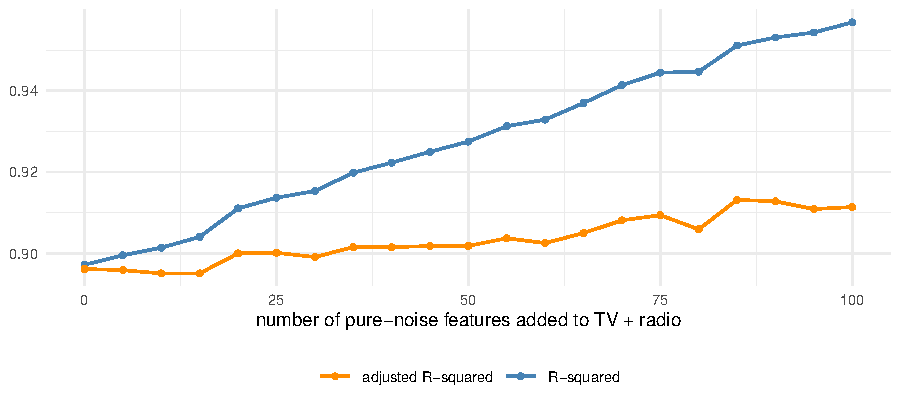
\includegraphics[width=0.95\linewidth]{figures/reg_junk_r2.pdf}
    \end{center}
\end{frame}

\mode<article>{
    \paragraph{Why the threshold is $|t| > 1$.}
    Let $\mathrm{RSS}_{\text{old}}$ be the residual sum of squares before adding one feature and $\mathrm{RSS}_{\text{new}}$ afterwards, with $p$ features in the old model. Then $R^2_{\text{adj}}$ increases if and only if $\mathrm{RSS}_{\text{new}}/(n-p-2) < \mathrm{RSS}_{\text{old}}/(n-p-1)$. Rearranging, this is $1 < (\mathrm{RSS}_{\text{old}} - \mathrm{RSS}_{\text{new}})(n-p-2)/\mathrm{RSS}_{\text{new}}$, and the right-hand side is the partial $F$-statistic of the added feature, which equals its squared $t$-statistic.
}

\begin{frame}{Comparing regression models on the Advertising data}
    \begin{center}
        \small
        \begin{tabular}{lrrrrr}
            \toprule
            model & RSE & RMSE & MAE & $R^2$ & adjusted $R^2$ \\
            \midrule
            TV & 3.259 & 3.242 & 2.550 & 0.6119 & 0.6099 \\
            TV + radio & 1.681 & 1.669 & 1.254 & 0.8972 & 0.8962 \\
            TV + radio + newspaper & 1.686 & 1.669 & 1.252 & 0.8972 & 0.8956 \\
            TV $\times$ radio & 0.944 & 0.934 & 0.660 & 0.9678 & 0.9673 \\
            \bottomrule
        \end{tabular}
    \end{center}
    \begin{itemize}
        \item RMSE and MAE are in thousands of units of sales: the typical error falls from about 3.2 (TV only) to about 0.9 (TV $\times$ radio)
        \item Adding newspaper leaves $R^2$ unchanged (0.8972) but lowers adjusted $R^2$ (0.8962 to 0.8956) and raises RSE: the penalty exposes a useless feature
        \item All numbers here are computed on the training data used to fit the models
    \end{itemize}
\end{frame}

\begin{frame}[allowframebreaks]{Training error versus test error}
    \begin{columns}[T]
        \begin{column}{0.55\textwidth}
            \begin{itemize}
                \item \textbf{Training MSE}: $\frac{1}{n} \sum_i \big(y^{(i)} - \hat{f}(\mathbf{x}^{(i)})\big)^2$ on the data used to fit $\hat{f}$; all earlier measures are training measures
                \item \textbf{Test MSE}: the same average over new observations not used in fitting
                \item More features always lower the training MSE; once the informative ones are in, the rest fit noise and the test MSE rises: \textbf{overfitting}
                \item Simulation: 50 observations, 45 features, 5 informative
            \end{itemize}
        \end{column}
        \begin{column}{0.43\textwidth}
            % ---- R code: figures/reg_train_test.pdf ----
            % library(tidyverse)
            % theme_set(theme_minimal(base_size = 9) +
            %             theme(plot.title = element_text(size = 9, face = "bold"),
            %                   plot.background = element_rect(fill = "transparent", colour = NA),
            %                   panel.background = element_rect(fill = "transparent", colour = NA),
            %                   legend.background = element_rect(fill = "transparent", colour = NA)))
            % dir.create("figures", showWarnings = FALSE)
            %
            % # training vs test MSE as features are added: 45 candidate features, only 5 matter
            % set.seed(2)
            % n_train <- 50; n_test <- 2000; n_feat <- 45; sigma <- 1
            % beta <- c(2, -1.5, 1, 1, -1, rep(0, n_feat - 5))          # only the first five features matter
            %
            % sim_data <- function(n) {
            %   X <- matrix(rnorm(n * n_feat), n, n_feat, dimnames = list(NULL, paste0("x", 1:n_feat)))
            %   as_tibble(X) |> mutate(y = drop(X %*% beta) + rnorm(n, sd = sigma))
            % }
            % train_df <- sim_data(n_train)
            % test_df <- sim_data(n_test)
            %
            % err <- map_dfr(1:n_feat, function(k) {
            %   fit <- lm(reformulate(paste0("x", 1:k), response = "y"), data = train_df)
            %   tibble(features = k, training = mean(resid(fit)^2),
            %          test = mean((test_df$y - predict(fit, test_df))^2))
            % }) |> pivot_longer(c(training, test), names_to = "set", values_to = "mse")
            %
            % p <- ggplot(err, aes(features, mse, colour = set)) +
            %   geom_line(linewidth = 0.6) +
            %   geom_hline(yintercept = sigma^2, linetype = "dashed") +
            %   annotate("text", x = 45, y = sigma^2, label = "irreducible error", vjust = -0.6, hjust = 1, size = 2.5) +
            %   coord_cartesian(ylim = c(0, 10)) +
            %   labs(title = "nested linear models, simulated data", x = "number of features used",
            %        y = "MSE", colour = NULL) +
            %   theme(plot.title = element_text(size = 8, face = "bold"))
            % ggsave("figures/reg_train_test.pdf", p, width = 3.4, height = 2.75, bg = "transparent")
            \begin{center}
                
\includegraphics[width=\linewidth]{figures/reg_train_test.pdf}
            \end{center}
        \end{column}
    \end{columns}
\end{frame}

\begin{frame}{Summary}
    \begin{itemize}
        \item \textbf{Residuals}: $\mathbf{e} = (\mathbf{I} - \mathbf{H})\symbf{\varepsilon}$ with $\mathrm{Var}(e^{(i)}) = \sigma^2 (1 - h^{(i)})$; standardized residuals $r^{(i)} = e^{(i)}/(\hat\sigma\sqrt{1-h^{(i)}})$
        \item \textbf{Diagnostics}: residual plots reveal non-linearity, correlated errors and non-constant variance; standardized residuals flag outliers, leverage flags unusual feature values, VIF flags collinearity
        \item \textbf{Performance}: MSE, RMSE, MAE, RSE, $R^2$ and adjusted $R^2$ measure the fit to the training data; RSE and adjusted $R^2$ account for the degrees of freedom
        \item \textbf{Training vs test}: training error keeps falling as features are added, test error does not
    \end{itemize}
\end{frame}